\documentclass[11pt,letterpaper]{article}
\usepackage[T1]{fontenc}
\usepackage{lmodern}
\usepackage[margin=0.9in]{geometry}
\usepackage{amsmath,amssymb,amsthm,mathtools}
\usepackage{booktabs,longtable,tabularx,array}
\usepackage{microtype,xcolor,enumitem,fancyhdr}
\usepackage{hyperref,xurl,pdfpages}
\hypersetup{colorlinks=true,linkcolor=blue!45!black,urlcolor=blue!55!black,
  citecolor=blue!45!black,pdftitle={A first Pell root eliminates an index quotient},
  pdfauthor={AI-assisted research prepared for Vladimir Reshetnikov}}
\pdfinfoomitdate=1
\pdftrailerid{}
\setlength{\parindent}{0pt}
\setlength{\parskip}{0.45em}
\setlength{\headheight}{14pt}
\setlength{\emergencystretch}{2em}
\pagestyle{fancy}
\fancyhf{}
\fancyhead[L]{\small A smaller consistency equation}
\fancyhead[R]{\small Pell root and index quotient}
\fancyfoot[C]{\thepage}
\newtheorem{theorem}{Theorem}[section]
\newtheorem{lemma}[theorem]{Lemma}
\newtheorem{proposition}[theorem]{Proposition}
\newtheorem{corollary}[theorem]{Corollary}
\theoremstyle{definition}
\newtheorem{definition}[theorem]{Definition}
\newtheorem{remark}[theorem]{Remark}
\newcommand{\Z}{\mathbb Z}
\newcommand{\N}{\mathbb N}
\newcommand{\Zp}{\mathbb Z_{>0}}
\newcommand{\ZFC}{\mathsf{ZFC}}
\newcommand{\Con}{\operatorname{Con}}
\newcommand{\fl}[1]{\left\lfloor#1\right\rfloor}
\newcommand{\code}[1]{\texttt{\small #1}}
\newcommand{\repo}{https://github.com/VladimirReshetnikov/ProveIt}
\newcommand{\sourcepin}{02a78a08603cbae248c19c23a75907c6c6bd6443}
\title{\textbf{A first Pell root eliminates an index quotient}\\[0.5em]
  \large A complete equation for syntactic ZFC consistency\\
  in fourteen positive variables, sixty-five operations, and degree 150}
\author{Research prepared for Vladimir Reshetnikov and ProveIt\\
  \small AI-assisted construction with independent internal mathematical review}
\date{25 October 2026}

\begin{document}
\maketitle
\thispagestyle{empty}

\begin{abstract}
The maintained admissible942 equation in ProveIt has fifteen positive integer
unknowns, sixty-six binary arithmetic operations, and exact total degree 157.
We remove an index quotient by making the existing first Pell root carry its
congruence. The substitution is
\(\tau=En+k-R\), with one new positive unknown \(n\) replacing the two old
unknowns \(h,\tau\); the factor \(k-hE-R\) disappears. A noncircular sign and
size argument recovers the omitted positive quotient from every new zero.
Canonical parent zeros give new zeros explicitly. The resulting polynomial
has fourteen positive unknowns, sixty-five integer-leaf operations, and exact
degree 150, with precisely the same four fixed integer coefficients.

A second, independent construction stores old transition targets as
reverse-discovery distances. One mixed-radix formula handles old targets,
new targets, and the early halt. It shortens the fully specified transition
numeral from 436 to 399 base-62 characters without changing any of the 430
actions, 942 indexed tiles, or four coefficient integers.

Composing the new arithmetic proof with the identified, pinned
P66/native/refutation calibration gives, in ZFC, equivalence between absence
of positive zeros and \(\Con(\ZFC)\). This is an ordinary mathematical proof,
not a new end-to-end Lean or Rocq verification. The archive contains the
complete one-page specification, all coefficient bytes, literal arithmetic
programs, independent finite checks, and domain translations. The result is
a strict improvement of the matched parent, not a global minimality claim.
\end{abstract}

\vfill
\begin{center}
\begin{tabular}{lrrr}
\toprule
Matched construction & Positive unknowns & Binary operations & Degree\\
\midrule
Pinned parent & 15 & 66 & 157\\
\textbf{This construction} & \textbf{14} & \textbf{65} & \textbf{150}\\
\bottomrule
\end{tabular}
\end{center}
\vfill
\clearpage
\setcounter{tocdepth}{1}
\tableofcontents
\clearpage

\section{Result, interpretation, and comparison}

The target is syntactic consistency: no finite formal derivation of a
contradiction exists in the effective ZFC presentation used by ProveIt's
retained calibration. No consistency assumption is made in proving an
equivalence with this statement.

\begin{theorem}[Main result]\label{thm:main}
Let \(P_{65}\in\Z[J,F,\alpha,z,f,i,T,s,w,n,\eta,\zeta,y,\gamma]\) be the
polynomial specified in Sections~\ref{sec:equation} and~\ref{sec:constants}.
Composing the arithmetic reduction proved here with the pinned parent
calibration yields
\[
 \ZFC\vdash
 \left[
   \left(\forall \mathbf x\in\Zp^{14}\right)P_{65}(\mathbf x)\ne0
 \right]\ \longleftrightarrow\ \Con(\ZFC).
\]
Its total degree is exactly \(150\). Its displayed arithmetic program
uses \(65\) binary operations with integer leaves: \(37\) multiplications,
\(16\) additions, and \(12\) subtractions.
\end{theorem}

The proof has two explicit layers. The new layer is a uniform elementary
arithmetic transformation, proved in full below. The inherited layer is the
particular parent's native encoding and its K215/syntactic-refutation
calibration. Copies of the immediate mathematical contracts and their exact
source identities are included. This report does not replace that inherited
development with a fresh proof-assistant build.

All repository comparisons in this report use the immutable commit
\[
 \texttt{\small 02a78a08603cbae248c19c23a75907c6c6bd6443}.
\]
The relevant parent is the complete \emph{admissible942} specialization,
not an earlier numerical tuple with the same arithmetic template
\cite{current,native}. The four large integers are preserved pointwise.
In particular, no mixture of coefficient ports from different historical
native encodings is used.

There are several meaningful size measures. The primary result improves
the matched parent's variable count, operation count, and degree
simultaneously. It does not minimize any of these among all possible
representations. The pinned repository already contains fewer-variable
equations with greater degree or cost, as well as direct proof-calculus
quartics with small coefficients \cite{collection,direct}. Small-variable
representation theorems in the literature provide further, different
benchmarks \cite{MR,Sun}.

An operation here is one binary \(+,-,\times\); a square costs one
multiplication. Fixed integer leaves and reuse of earlier registers cost
zero operations. This is an arithmetic-circuit measure, not bit complexity:
the four fixed integers require \(94\,689\) unsigned bytes in total.
Their complete finite recipe is printed rather than hidden behind an
unspecified universal-polynomial parameter.

\section{The complete polynomial}\label{sec:equation}

The independent unknowns, in their evaluator order, are exactly
\[
 \boxed{J,F,\alpha,z,f,i,T,s,w,n,\eta,\zeta,y,\gamma\in\Zp.}
\]
The four fixed positive integers are \(\beta,K,M_C,M_F\), defined in
Section~\ref{sec:constants}. All other symbols in this section are
polynomial abbreviations and are not additional unknowns.

Define
\begin{align}
 q_-&=\beta J,& q&=q_-+1,& C&=q-F-\alpha,\label{eq:q}\\
 X&=wq,&Y&=sq^3,&E&=XY,\label{eq:XY}\\
 k&=\eta+\zeta,&\ell&=EkY,&c&=kY+\eta,\label{eq:k}\\
 a&=E+Y,& H&=4a+3,&\Delta&=a^2+H,\label{eq:delta}\\
 D&=X+ac+\gamma H.&&&&\label{eq:D}
\end{align}
Then put
\begin{align}
 R&=\bigl[q_-(q-F)+\alpha\bigr](q^2-1)+(M_C+qM_F)J,\label{eq:R}\\
 \tau&=En+k-R,\label{eq:carrier}\\
 V&=f^2(cT-R)-c,& S&=i\Delta c^2.\label{eq:VS}
\end{align}
The five factors are
\begin{align}
 N_0&=\tau^2-\ell(\ell+k),&
 N_1&=D^2-\Delta c^2,\label{eq:norms}\\
 N_a&=S^2(V^2-y^2)+y^2,\label{eq:aux}\\
 N_t&=(K+w)C+(q-F)-zq_-,&
 N_s&=\Delta f^2-S^2.\label{eq:transport}
\end{align}
The requested single equation is
\begin{equation}\label{eq:final}
 \boxed{P_{65}:=N_0N_1N_aN_tN_s-\Delta=0.}
\end{equation}

Every exponent involving the fourteen unknowns is a fixed nonnegative
integer. Equation~\eqref{eq:final} is therefore an ordinary polynomial
equation over \(\Z\). The finite sums, floors, remainders, and powers used
later describe fixed coefficients only; none is an additional operation
on a Diophantine unknown.

\section{The exact inherited interface}\label{sec:interface}

The parent \(P_{66}\) uses the same definitions except that \(h,\tau\) are
independent positive unknowns and \(n\) is absent. It includes
\[
 N_k=k-hE-R
 \qquad\text{and}\qquad
 P_{66}=N_0N_1N_aN_kN_tN_s-\Delta.
\]
The immediate sources are the current complete equation
\cite{current}, the full admissible942 proof \cite{native}, and the uniform
positive P66 argument \cite{P66}. The latter is historically presented
with another tuple; its uniform arithmetic interface is used only after
the current native theorem supplies the complete current specialization.

We use two consequences of that retained calibration:
\begin{enumerate}[label=(\roman*),leftmargin=2em]
 \item Every positive zero of the current \(P_{66}\) produces a finite
 syntactic ZFC refutation.
 \item Every finite syntactic ZFC refutation produces a canonical positive
 zero with
 \[
 N_0=N_1=N_a=N_k=N_t=1,\qquad
 f^2-\Delta i^2c^4=1,\qquad R>0.
 \]
\end{enumerate}
These are mathematical source theorems, not assumptions that ZFC is
consistent or inconsistent. The new transformation needs only these
two directions. It does not need the stronger claim that all parent
zeros satisfy the canonical sign conditions.

The new argument uses the following simple scalar properties:
\begin{equation}\label{eq:boxes}
 \beta\ge31,\qquad K>0,\qquad 0<M_C<\beta<M_F<2\beta.
\end{equation}
Here \(M_F\) is the \emph{source} mask, including the inherited single
\(\beta\) shift. The supplied coefficient checker verifies
\eqref{eq:boxes} on the full actual integers and compares their canonical
bytes with the pinned certificate.

The parent's native theorem has additional geometric, mask, and controller
content. We do not attempt to replace those premises by the scalar boxes.
The boxes suffice for the \emph{new arithmetic reduction}; the complete
current native theorem supplies the meaning of the fixed coefficients.
Since all four integers are unchanged, the parent's finite controller
certificate is unchanged too.

\section{An elementary Pell lemma}\label{sec:pell}

The useful structure is the first norm, before the later norm-combining
steps. Its discriminant is the product of consecutive integers.

\begin{lemma}[Consecutive-product Pell equations]\label{lem:pell}
Let \(m\ge2\) be an integer and let \(d=m(m+1)\).
\begin{enumerate}[label=(\alph*),leftmargin=2em]
 \item The equation \(x^2-dy^2=-1\) has no integer solution.
 \item Every solution of \(x^2-dy^2=1\) with \(x,y>0\) has
 \[
 x=\chi_{2m+1}(r),\qquad y=2\psi_{2m+1}(r),\qquad r\ge1,
 \]
 where
 \[
 \chi_A(r)+\psi_A(r)\sqrt{A^2-1}
      =(A+\sqrt{A^2-1})^r.
 \]
 \item If \(E\mid m\), then \(x\equiv1\pmod E\). At \(r=1\) one has
 \(y=2\); at \(r\ge2\) one has \(y\ge4(2m+1)\). Also \(x>y\).
\end{enumerate}
\end{lemma}

\begin{proof}
For (a), a solution has \(y\ne0\). Choose one with least positive
\(|y|\), and replace \(x,y\) by their absolute values. Since
\(x^2=d y^2-1\), the inequalities
\[
 my<x<(m+\tfrac12)y
\]
follow by squaring: \(my^2>1\) and
\((m+\tfrac12)^2-d=\tfrac14\). The integer transformation
\[
 x'=(2m+1)x-2dy,\qquad y'=(2m+1)y-2x
\]
preserves the norm because \((2m+1)^2-4d=1\). The displayed bounds
give \(0<y'<y\). Taking \(|x'|\) if necessary produces a smaller
solution of norm \(-1\), a contradiction.

For (b), no solution has \(y=1\), since
\[
 m^2<d+1<(m+1)^2.
\]
For \(y\ge2\), norm one implies
\[
 my<x\le(m+\tfrac12)y.
\]
The same transformation gives \(0\le y'<y\). Its first coordinate
is positive: squaring the two positive terms gives
\[
 (2m+1)^2x^2-4d^2y^2=d y^2+4d+1>0.
\]
Descent terminates at \((1,0)\). Reversing it proves that every solution
is a positive power of
\((2m+1)+2\sqrt d\). Since
\((2m+1)^2-1=4d\), this is the claimed parametrization.

For (c), the first coordinate satisfies the integer recurrence
\[
 \chi_A(0)=1,\quad \chi_A(1)=A,\quad
 \chi_A(r+1)=2A\chi_A(r)-\chi_A(r-1).
\]
If \(A=2m+1\equiv1\pmod E\), induction gives
\(\chi_A(r)\equiv1\pmod E\). The second coordinates begin
\(\psi_A(1)=1\), \(\psi_A(2)=2A\) and strictly increase.
Finally \(x^2=1+dy^2>y^2\).
\end{proof}

This proof is elementary integer arithmetic and induction. The apparent
real square roots merely abbreviate the equivalent pair recurrences.
Thus no external-standardness or real-analysis assumption is needed
when formalizing it in ZFC.

\section{Recovering all unit signs before using the new root}

Fix an arbitrary positive zero of \(P_{65}\). We first recover signs
without assuming that its polynomial abbreviation \(\tau\) is positive.
This order is essential: \(\tau\) is no longer an independent positive
coordinate.

For every positive assignment,
\[
 q\ge32,\quad X,Y,E,a,c>0,\qquad
 \Delta=(a+2)^2-1>0.
\]
Moreover,
\[
 N_s=\Delta\,U_s,\qquad
 U_s=f^2-\Delta(i c^2)^2.
\]
Cancelling the nonzero \(\Delta\) in \(P_{65}=0\) gives
\begin{equation}\label{eq:unitprod}
 N_0N_1N_aN_tU_s=1.
\end{equation}
Each of the five integer factors is consequently \(+1\) or \(-1\).

Since \(\ell=EkY\), putting \(m=EY\ge2\) gives
\[
 N_0=\tau^2-m(m+1)k^2.
\]
Lemma~\ref{lem:pell}(a) excludes \(N_0=-1\), even if \(\tau\)
has not yet been shown positive.

The value of \(\Delta\) is \(0\) or \(3\) modulo four. A square minus
\(\Delta\) times a square cannot be \(3\) modulo four. Therefore
\[
 N_1\ne-1,\qquad U_s\ne-1.
\]
For the remaining norm, if \(S\) is even then \(N_a\equiv y^2\pmod4\);
if \(S\) is odd then \(N_a\equiv V^2\pmod4\). Thus \(N_a\ne-1\).
Equation~\eqref{eq:unitprod} now forces the only remaining sign:
\begin{equation}\label{eq:allunits}
 \boxed{N_0=N_1=N_a=N_t=U_s=1.}
\end{equation}

The old product had two unresolved linear signs, \(N_k,N_t\).
Removing \(N_k\) has a useful additional effect: it makes \(N_t=1\)
available immediately. This is what permits the following size estimates
without assuming the missing quotient in advance.

\section{Rank bounds and recovery of the positive quotient}

\subsection{Bounds derived directly from transport}

Suppose \(C\le0\). Since \(K+w>0\), \(F,z\ge1\), and \(q_-=q-1\),
\[
 N_t=(K+w)C+(q-F)-z(q-1)
       \le(q-1)-z(q-1)\le0.
\]
This contradicts \(N_t=1\), so \(C>0\).

Write \(u=q-F=C+\alpha\). Positivity gives
\[
 2\le u\le q-1,\qquad 1\le\alpha\le u-1.
\]
Consequently
\[
 2q-1\le G:=(q-1)u+\alpha\le q^2-q-1.
\]
By the coefficient boxes \eqref{eq:boxes} and \(\beta J=q-1\),
\[
 0<(M_C+qM_F)J<(1+2q)(q-1).
\]
Substitution into \eqref{eq:R} yields
\begin{equation}\label{eq:Rbounds}
 q(q^2-1)<R<q^4-q^3.
\end{equation}
For the upper bound the cancellation is exact:
\[
 (q^2-q-1)(q^2-1)+(1+2q)(q-1)=q^4-q^3.
\]
Also \(E=wsq^4\ge q^4\). Thus \(R>1\), \(R+2<E\), and
\begin{equation}\label{eq:taupositive}
 \tau=En+k-R\ge E+k-R>k+2>0.
\end{equation}
No part of this argument used an old \(h\) coordinate.

\subsection{The missing divisibility condition}

Apply Lemma~\ref{lem:pell} to \(N_0=1\). Since \(k=\eta+\zeta>0\)
and \(\tau>0\), there is \(r\ge1\) with
\[
 \tau=\chi_{2EY+1}(r),\qquad k=2\psi_{2EY+1}(r).
\]
As \(E\mid EY\), we obtain
\[
 \tau\equiv1\pmod E.
\]
The definition \(\tau=En+k-R\) therefore proves
\[
 E\mid k-R-1.
\]
Define, in the proof only,
\begin{equation}\label{eq:restoreh}
 h=\frac{k-R-1}{E}.
\end{equation}
This is an integer. Since \(R+1<E\) and \(k>0\), it is greater than
\(-1\), hence nonnegative.

It remains to prove strict positivity. If \(h=0\), then
\(k=R+1<E\). At Pell index \(r=1\), however, \(k=2\) would give
\(R=1\), contradicting \eqref{eq:Rbounds}. At \(r\ge2\),
\[
 k\ge4(2EY+1)>E,
\]
again a contradiction. Therefore \(h>0\), and
\begin{equation}\label{eq:Nkone}
 k-hE-R=1.
\end{equation}

\begin{proposition}[Soundness map]\label{prop:sound}
Every positive zero of \(P_{65}\) maps to a positive zero of the
pinned \(P_{66}\) by retaining the thirteen common coordinates and taking
\[
 \tau_{\rm old}=En+k-R,\qquad h_{\rm old}=(k-R-1)/E.
\]
\end{proposition}
\begin{proof}
Both inserted coordinates are positive integers by the preceding argument.
Every retained abbreviation and norm has exactly its new value, and
the restored factor \(N_k\) is one. The parent product therefore equals
the new product, namely \(\Delta\).
\end{proof}

\section{Completeness and the internal consistency equivalence}

Start with a finite syntactic refutation. The inherited canonical
completeness theorem supplies a positive parent zero with
\(N_k=N_t=1\), \(N_0=1\), and \(R>0\).
Lemma~\ref{lem:pell} gives
\[
 \tau_{\rm old}\equiv1\pmod E,\qquad \tau_{\rm old}>k.
\]
Since \(N_k=1\), \(k-R\equiv1\pmod E\). Hence
\begin{equation}\label{eq:restoren}
 n=\frac{\tau_{\rm old}-k+R}{E}
\end{equation}
is a positive integer. It satisfies \(En+k-R=\tau_{\rm old}\).
All five retained factors have their canonical values, so \(P_{65}=0\).

Combining this construction with Proposition~\ref{prop:sound} and the
parent soundness theorem gives the two implications
\[
 \exists\mathbf x\in\Zp^{14}\ P_{65}(\mathbf x)=0
 \quad\Longleftrightarrow\quad
 \exists p\ \operatorname{Refutation}_{\ZFC}(p).
\]
Negation proves Theorem~\ref{thm:main}. The proof is a composition of
arithmetical statements and explicit witness transformations. It is
internal to ZFC: the proof variable \(p\) ranges over the theory's natural
numbers, rather than an externally selected set of standard codes.

The existence proof does not assert that every parent zero is already
canonical. If the retained stronger all-zero sign-recovery theorem is
also invoked, \eqref{eq:restoreh} and \eqref{eq:restoren} give mutually
inverse maps on the full positive zero sets. That stronger conclusion
is optional and is not needed for the consistency equivalence.

This argument neither proves nor refutes \(\Con(\ZFC)\). In particular,
the certificate checks in the archive do not search for a refutation or
for a zero. They authenticate the specified finite arithmetic data.

\section{Exact cost and degree}\label{sec:metrics}

\subsection{The arithmetic program}

The parent computes \(N_k\) with three operations:
\[
 hE,\qquad k-hE,\qquad k-hE-R.
\]
It uses one further multiplication to include \(N_k\) in the output.
All four operations disappear. The new root costs exactly three:
\[
 En,\qquad En+k,\qquad En+k-R.
\]
The remaining registers can be scheduled in the old dependency order
after moving the first norm below the definition of \(R\). Thus
\[
 66-3-1+3=\boxed{65}.
\]
The literal program in Appendix~\ref{app:gates} has no division, rational
constant, dead register, or unused input. Its operator split is
\(37\) multiplications, \(16\) additions, and \(12\) subtractions.

\subsection{Why the degree is exactly 150}

Assign degree one to each unknown and degree zero to each fixed integer.
The important degrees are:
\begin{center}
\begin{tabular}{lrrrrrrrr}
\toprule
Quantity & \(q\)&\(X\)&\(Y\)&\(E\)&\(k\)&\(c\)&\(\ell\)&\(\tau\)\\
\midrule
Degree &1&2&4&6&1&5&11&7\\
\bottomrule
\end{tabular}
\end{center}
The first norm retains degree \(22\), since the new \(\tau^2\) has
degree \(14\), less than that of \(\ell^2\).

The main norm requires an actual cancellation calculation. Put
\(Z=X+\gamma H\). Then
\begin{equation}\label{eq:n1cancel}
 N_1=(ac+Z)^2-(a^2+H)c^2
       =2acZ+Z^2-Hc^2.
\end{equation}
Its degree is \(18\), rather than the naive upper bound \(22\).
The five exact factor degrees are
\begin{center}
\begin{tabular}{lrrrrr}
\toprule
Factor & \(N_0\)&\(N_1\)&\(N_a\)&\(N_t\)&\(N_s\)\\
\midrule
Exact degree &22&18&62&2&46\\
\bottomrule
\end{tabular}
\end{center}
Their sum is \(150\), while \(\deg\Delta=12\).

For a direct noncancellation certificate, write
\(q_0=\beta J\), \(k_0=\eta+\zeta\). The complete highest homogeneous
part is
\begin{equation}\label{eq:leader}
\begin{split}
 L_{150}={}&8q_0^{87}\gamma i^4 k_0^{13}w^{12}s^{25}T^2f^4\\
 &{}\cdot\bigl[w(q_0-F-\alpha)-zq_0\bigr].
\end{split}
\end{equation}
In particular, the coefficient of
\[
 J^{88}z\gamma i^4\eta^{13}w^{12}s^{25}T^2f^4
\]
is \(-8\beta^{88}\ne0\). This proves the exact degree at the actual
fixed tuple, rather than only at generic formal coefficient parameters.

The arithmetic checker independently expands the entire main-norm
ancestor cone, obtaining \(323\) terms, and compares all \(56\) terms
of \eqref{eq:leader}. The independent checker also verifies the
displayed formula identities and a full univariate specialization of
degree \(150\). The latter is a finite cross-check; the proof of the
global upper bound and the actual nonzero coefficient is the argument
above.

\section{The four fixed integers and their complete finite recipe}
\label{sec:constants}

\subsection{Masks and kernel}

Set
\[
 \rho=2^{47},\qquad B=\rho^{4027},\qquad\beta=B-1,\qquad
 G_m(x)=\sum_{j=0}^{m-1}x^j,\qquad
 \Lambda=\rho^{1992}+\rho^{2998}.
\]
Define
\begin{align}
 \Psi(x,t)
   &=x^{969}(x^9+t^{17})G_8(tx)
     +t^8x^{942}(x^{18}+t^{17})G_9(tx)
     +(2-t)x^{1005},\label{eq:Psi}\\
 \Phi(x)
   &=\sum_{j=0}^{941}
       \bigl[1+2^{10}(1+w_j+2^8n_j+2^{17}p_j+2^{25}s_j)\bigr]x^j
       +2^{10}\Psi(x,2).\label{eq:Phi}
\end{align}
The indexed tuples \((w_j,n_j,p_j,s_j)\) are specified below.
The remaining three constants are
\begin{align}
 M_C={}&\beta-\rho^{977}-G_{942}(\rho)-\Psi(\rho,1),\label{eq:MC}\\
 M_F={}&B+3+(2^{44}-2)\Lambda
       +\rho^{960}G_9(\rho)+\rho^{987}G_8(\rho)+\rho^{1005}\notag\\
       &\hspace{3em}+2^{27}\rho^{4022}-\rho^{4004},\label{eq:MF}\\
 K={}&\rho^{18}+\rho^{1005}+\rho^{4036}
            +\Lambda\Phi(1/\rho).\label{eq:K}
\end{align}
The last expression is an integer. Every exponent in \(\Phi\) is at
most \(1005\), while both exponents in \(\Lambda\) exceed \(1005\);
distributing the product removes every displayed negative power.

\subsection{The exact indexed tile table}

Let \(u_j,v_j,d_j\), for \(0\le j<430\), be the action data decoded in
the next subsection. Define, for \(d=0,1\),
\[
 h_0(q,b)=2q+b+2,\qquad
 \mathcal S_d=\{u_j:d_j=d,\ 0\le j<430\},
\]
\[
 r_{d,q}=205-199d+
       |\mathcal S_d\cap\{0,\ldots,q-1\}|.
\]
An interval ending at \(-1\) is empty. These definitions are finite
operations on fixed data. The tile at index \(i\) is the tuple
\(t_i=(w_i,n_i,p_i,s_i)\) in the following table.

\begin{center}
\small
\setlength{\tabcolsep}{4pt}
\begin{tabular}{@{}ll@{}}
\toprule
Index \(i\) & \(t_i=(w_i,n_i,p_i,s_i)\)\\
\midrule
\(0\) & \((2,435,3,1)\)\\
\(j+1,\ j=2q+b<430\)
 & \(((1-d_j)r_{0,u_j},h_0(q,b),d_jr_{1,u_j},v_j)\)\\
\(433-2a+b,\ a,b\in\{0,1\}\)
 & \((0,432a+b,0,432a+b)\)\\
\(423+2r_{d,q}+b\)
 & \((dr_{d,q},b,(1-d)r_{d,q},h_0(q,b))\)\\
\(\quad q\in\mathcal S_d,\ d,b\in\{0,1\}\)&\\
\(923+2a+b,\ a,b\in\{0,1\}\)
 & \((0,432a+b,0,438)\)\\
\(927\) & \((2,434,2,0)\)\\
\(928\) & \((3,436,4,4)\)\\
\(929\) & \((4,436,4,0)\)\\
\(496+t,\ t\in\{434,435,436\}\)
 & \((1,438,1,t)\)\\
\(933+3a+b,\ a,b\in\{0,1,2\}\)
 & \((a^2,437,b,437)\)\\
\bottomrule
\end{tabular}
\end{center}
The supplied finite reconstruction verifies that these formulas assign
each index \(0,\ldots,941\) exactly once. They retain the actual
initializer \(t_{928}=(3,436,4,4)\). The symbol \(h_0\) in this finite
table is unrelated to the quotient \(h\) removed from the polynomial.

\subsection{The new closed action decoder}

For \(b>0\), use the least nonnegative remainder and write
\[
 D_b(A,k)=\fl{A/b^k}\bmod b,\qquad
 A\bmod b=A-b\fl{A/b}.
\]
Let \(\mathcal A\) be the fully printed numeral below. Set
\[
 N=\mathcal A\bmod 2^{636},\qquad Q=\fl{\mathcal A/2^{636}}.
\]
For \(0\le j<430\), and for prefix quantities also at \(j=430\), put
\begin{align}
 \nu_j&=D_2(N,j),&
 \sigma_j&=\sum_{k<j}\nu_k,\label{eq:prefix}\\
 r_j&=(\sigma_j+2)^{1-\nu_j},&
 P_j&=\prod_{k<j}r_k.\label{eq:radices}
\end{align}
Thus \(\sigma_0=0\), \(P_0=1\); an empty sum is zero and an empty
product is one.

For \(0\le q<215\), \(b\in\{0,1\}\), \(j=2q+b\), define
\begin{align}
 m_q&=D_2(N,430+q),&
 \theta_q&=\sum_{k<q}m_k,\label{eq:mask}\\
 F_q&=14+m_q\left(D_{16}\!\left(\fl{Q/P_{430}},\theta_q\right)-14\right),
   \label{eq:flags}\\
 u_j&=\left(\sigma_{j+1}
        -\left(\fl{Q/P_j}\bmod r_j\right)\right)\bmod216,\label{eq:target}\\
 v_j&=D_2(F_q,2b),&
 d_j&=D_2(F_q,2b+1).\label{eq:write}
\end{align}
Every radix \(r_j\) is positive. At a discovery it equals one, and
reduction modulo one is well-defined and equals zero. There is no
circular dependence: \(N\) determines all discovery bits, which
determine all prefix products, after which the flag field and targets
are decoded.

\subsection{The complete 399-character numeral}

The digit alphabet, in order of values \(0,\ldots,61\), is
\[
 \texttt{\small 0123456789ABCDEFGHIJKLMNOPQRSTUVWXYZabcdefghijklmnopqrstuvwxyz}.
\]
Concatenate the following seven lines into digits
\(e_0,\ldots,e_{398}\), and set
\(\mathcal A=\sum_{j=0}^{398}e_j62^{398-j}\).
\begin{quote}
\ttfamily\small
5TPXx0McEgSbYki3sGVNKJLlN8Q3rCXEfmrabEMMQ8k2o7MWvDH3pCkVAr7WqE\\
SjjWJ6dfq6LXnsZ6OHq7X5iVUPDlwMCAVZSQetoQ0ToXWH6MDnc00LmAYqNDjl\\
4vOt5Pyqlm1w3QNJbgusSWi8PpjYYL0GfwYX6CiaBwhYAamgcErq0NvxD1RlnG\\
hk2ZQlIzR5QYJ7qPAGs4LiKjiwLVxBklwY6mc0rXASKtPvKSExJCqmSq0QA4We\\
dyi3CmNTqaYAAUHXNKVii0Y7dPyuBGK3Wf9xU3vNHYczDPSJUREK7toNXVZLE0\\
Av8LC0sn6Z6b3e6vj2YEsfHM9lAXImUXzNvBajRskYaVHYhxtRPsiISO0Rst1h\\
16ymUkkXf1F2lVOfi8rCWgfBlPp
\end{quote}
This numeral, the displayed decoder, the indexed table, and
\eqref{eq:Psi}--\eqref{eq:K} completely specify the coefficients.
No lookup in the old 436-character numeral is part of the new
definition.

\subsection{Exact coefficient identities}

The coefficients reconstructed by this recipe equal the current
admissible942 coefficients as integers, not merely modulo a chosen
test modulus.
\begin{center}
\begin{tabular}{lrr}
\toprule
Coefficient & Bit length & Minimal unsigned bytes\\
\midrule
\(\beta\)&189\,269&23\,659\\
\(K\)&189\,693&23\,712\\
\(M_C\)&189\,269&23\,659\\
\(M_F\)&189\,270&23\,659\\
\midrule
Total&&94\,689\\
\bottomrule
\end{tabular}
\end{center}
The full byte identities are recorded in
\code{equation/coefficients.json}. The inherited certificate is copied
as \code{sources/admissible942\_certificate.json}. Thus the new numeral
does not create new controller or native-language obligations.

\section{Why reverse-discovery distances shorten the decoder}
\label{sec:seedproof}

The repository had already explored mixed-radix target packing
\cite{mixed}. Its smaller numerals did not automatically make a shorter
complete description: their decoding overhead could outweigh the saved
digits. The new component is the choice of stored digit.

\begin{lemma}[Reverse-discovery packing]\label{lem:packing}
Let active labels be \(0,\ldots,H-1\), with halt label \(H\), and
suppose \(m\) fixed actions discover the active states in order.
Write \(\nu_j\in\{0,1\}\) for a discovery and
\(\sigma_j=\sum_{k<j}\nu_k\), with \(\sigma_m=H-1\).
A discovery targets \(\sigma_j+1\); an old active target is at most
\(\sigma_j\). Define
\[
 r_j=(\sigma_j+2)^{1-\nu_j},\qquad
 P_j=\prod_{k<j}r_k.
\]
Store the digit
\[
 d_j=
 \begin{cases}
 0,&\nu_j=1,\\
 \sigma_j-u_j,&u_j\le\sigma_j\text{ is an old active target},\\
 \sigma_j+1,&u_j=H.
 \end{cases}
\]
Let \(T_*=\sum_{j<m}d_jP_j\), and let
\(Q_*=T_*+P_m E_*\) for any nonnegative auxiliary integer \(E_*\).
Then \(0\le T_*<P_m\), \(E_*=\fl{Q_*/P_m}\), and
\[
 u_j=
 \left(\sigma_{j+1}
     -\left(\fl{Q_*/P_j}\bmod r_j\right)\right)\bmod(H+1).
\]
\end{lemma}

\begin{proof}
Each digit satisfies \(0\le d_j<r_j\), including the radix-one discovery
case. Induction on the finite mixed-radix expansion gives
\(0\le T_*<P_m\). In extracting a digit at position \(j\), all earlier
terms sum to less than \(P_j\), while all later terms and the auxiliary
field are divisible by \(P_jr_j\). Thus the extracted remainder is
exactly \(d_j\).

At a discovery the subtraction gives \(\sigma_j+1\); at an old active
target it gives \(u_j\); at a halt it gives \(-1\), whose least
nonnegative residue modulo \(H+1\) is \(H\). These cases are exhaustive.
\end{proof}

For the actual table \(m=430\), \(H=215\). The low field \(N\) and the
exceptional write/move nibbles are unchanged. Only the target
representation changes:
\[
 \mathcal A_{\rm new}=N+2^{636}(T_*+P_{430}E_*).
\]
The unique halt occurs at action \(125\), after \(80\) discoveries.
Its stored digit is \(81\), so the unreduced target is \(-1\).
This explains why the outer modulo \(216\) in \eqref{eq:target} is
necessary.

The new numeral has \(2373\) bits and \(399\) base-62 characters, compared
with \(2594\) bits and \(436\) characters for its parent. The complete
specification, including decoding overhead, also becomes shorter in
the delivered template:
\begin{center}
\small
\begin{tabular}{lrr}
\toprule
Metric & Pinned parent & Combined new page\\
\midrule
Numeral characters &436&399\\
Coefficient recipe, nonwhite extracted characters &1992&1980\\
Whole page, same convention &2671&2655\\
Standalone TeX bytes &5025&5014\\
Pages &1&1\\
Words in local text extraction &738&743\\
Locally rebuilt PDF bytes &159\,737&160\,419\\
\bottomrule
\end{tabular}
\end{center}
The character convention is \code{pdftotext -raw}, followed by counting
nonwhite characters. It is not a glyph census. The gain includes the
inlined auxiliary flag field and the shorter explicit empty-sum/product
convention. Word count and PDF byte size increase; no improvement in
those metrics is claimed. The repository's stored parent PDF had
\(159\,721\) bytes; the table compares both pages rebuilt in the same
local environment.

\section{Natural and unrestricted integer versions}
\label{sec:domains}

The witness domain is part of the theorem. Merely allowing arbitrary
integers in the fourteen-variable expression would not preserve the
argument above.

\subsection{Fourteen nonnegative variables}

For each old positive variable \(v\), substitute \(v=u_v+1\) with
\(u_v\in\N=\{0,1,\ldots\}\). This gives a completely specified polynomial
\(P_{\N}\) in fourteen nonnegative unknowns. The translation is bijective
on domains, so the zero-existence equivalence is immediate.
Its degree is exactly \(150\); adding constants does not alter the
highest homogeneous part. A literal evaluator uses \(65+14=79\)
operations. It is supplied as \code{equation/natural14.json}.

\subsection{Forty-two unrestricted integer variables}

Use, independently for each of the fourteen variables, the substitution
\begin{equation}\label{eq:onto}
 v=1+a_v^2+b_v^2+c_v(c_v+1),
 \qquad a_v,b_v,c_v\in\Z.
\end{equation}
Its value is always positive. It is onto \(\Zp\): for \(v\ge1\),
Legendre's three-square theorem represents
\(4(v-1)+1\) as three integer squares, since that number is not of
the exceptional form \(4^a(8b+7)\). Reduction modulo four shows exactly
one of the squares is odd. Relabeling the coordinates gives
\[
 4(v-1)+1=(2a_v)^2+(2b_v)^2+(2c_v+1)^2,
\]
which is equivalent to \eqref{eq:onto}.

Consequently the single ordinary integer equation
\[
 \boxed{P_{\Z}((a_v,b_v,c_v)_v)
       :=P_{65}\bigl((1+a_v^2+b_v^2+c_v(c_v+1))_v\bigr)=0}
\]
has an integer zero exactly when \(P_{65}\) has a positive zero.
This supplies an unrestricted-integer formulation of the requested
consistency equivalence with \(42\) unknowns.

Each substitution costs seven binary operations, so the literal program
uses \(65+14\cdot7=163\) operations. Its exact degree is \(300\).
To see that the highest part cannot vanish, take the nonzero
\(L_{150}\) in \eqref{eq:leader} and replace each variable by
\(a_v^2+b_v^2+c_v^2\). Setting all \(b_v,c_v\) to zero maps distinct
old monomials to distinct doubled-exponent monomials in the \(a_v\)'s;
the substitution is injective. The resulting degree-\(300\) form is
therefore nonzero.

\begin{center}
\begin{tabular}{lrrr}
\toprule
Witness domain & Unknowns & Operations & Exact degree\\
\midrule
Strictly positive integers &14&65&150\\
Nonnegative integers &14&79&150\\
Unrestricted integers &42&163&300\\
\bottomrule
\end{tabular}
\end{center}
The last graph is \code{equation/integer42.json}. These domain
translations are supplied for completeness, not as new low-variable
records over \(\Z\).

\section{Verification, reproducibility, and proof boundaries}
\label{sec:verification}

\subsection{What the finite checks establish}

The archive's verifier uses Python 3.10 or later and the standard library.
It performs exact integer calculations and sparse polynomial identities.
The independent arithmetic checker imports no producer code.

The checks authenticate the pinned parent files; rebuild the three
literal equation graphs and all four coefficient files; compare all
430 actions and 942 indexed tiles; verify the complete coefficient
integers; check the new scalar interface; count and inspect every
arithmetic register; verify the displayed formula identities; and
check exact total degree. A separately written decoder uses successive
quotient/remainder extraction instead of the author's prefix-floor
formula and reconstructs the printed numeral in reverse.

Deliberate changes to the trace sign, a product factor, the witness
domain, and three different numeral symbols are rejected. These checks
are concrete transcription safeguards. They do not replace the
unbounded proofs of Pell classification, the reconstruction of \(h\),
or the inherited logical calibration.

The mathematical checks were run normally and with Python optimization
enabled. Substantive conditions use explicit failures rather than
removable \code{assert} statements. The normal and optimized results
are retained in \code{verification/}. The one-page equation and this
report were compiled, rendered, and visually inspected.

\subsection{Reproduction commands}

From the extracted archive directory:
\begin{quote}\ttfamily\small
python3 -B verify.py\\
python3 -B -O verify.py\\
python3 -B code/build.py
\end{quote}
The first two commands are read-only. The third reconstructs the eight
equation/coefficient files in memory and compares them byte for byte.
To write a fresh reconstruction into a directory that does not exist:
\begin{quote}\ttfamily\small
python3 -B code/build.py --output-dir /tmp/conzfc-carrier-rebuilt
\end{quote}
To evaluate a supplied tuple, use a JSON array in the exact coordinate
order in the applicable equation graph:
\begin{quote}\ttfamily\small
python3 -B evaluate.py tuple.json\\
python3 -B evaluate.py --domain natural tuple.json\\
python3 -B evaluate.py --domain integer tuple.json
\end{quote}
Evaluation reports whether the exact value is zero, its sign, bit length,
and magnitude hash. The option \code{--value} prints the entire decimal
integer, which can be large. No evaluator performs a root search.

Rebuild the PDFs with a normal TeX installation:
\begin{quote}\ttfamily\small
pdflatex -interaction=nonstopmode -halt-on-error equation.tex\\
pdflatex -interaction=nonstopmode -halt-on-error report.tex\\
pdflatex -interaction=nonstopmode -halt-on-error report.tex
\end{quote}
The report's last page includes the compiled one-page equation. Its full
formula and coefficient recipe also appear in the report source.
PDF metadata or font versions can change bytes after rebuilding.
Use \code{verify.py --skip-manifest} after an intentional PDF rebuild;
the exact arithmetic and coefficient comparisons remain active.

\subsection{What has and has not been newly proved}

The new, fully written mathematics consists of the first-root congruence
reduction, its noncircular sign and positivity proof, the exact cost and
degree calculation, and the reverse-discovery packing lemma. The domain
translations use standard number theory. Internal independent AI-assisted
reviews are included; they are not external human peer reviews.

The full native-to-refutation correspondence remains the identified
ProveIt theorem. The immediate proofs are copied with immutable source
identities, but the archive is not a complete Lean/Rocq dependency closure.
No new formal-kernel or object-language ZFC derivation has been compiled
in this iteration. These distinctions are explicit because a finite
coefficient checker cannot by itself establish the unbounded consistency
statement.

\section{Novelty assessment and the next useful direction}

The useful new mechanism is quite specific: preserve the \emph{bare}
first Pell root long enough to use the congruence it already carries.
The old first norm authenticates \(\tau\equiv1\pmod E\). An affine
change in that root turns the congruence into the old quotient condition
without a separate \(h\) variable or \(N_k\) factor. Removing that factor
also resolves the transport sign earlier, which makes the positivity
proof work.

Source170 already explores related quotient carriers in a combined Pell
root and adjusts auxiliary witnesses \cite{quotient}. The current
construction uses the first root itself and does not need that extra
scaling. The inspected current formulas and collection summaries did
not contain this exact \(14/65/150\) point. This is a bounded repository
novelty assessment, not a literature-wide priority theorem.

The reverse-discovery result likewise builds on an existing repository
idea. Mixed-radix compression was already known there; the new digit
choice removes a separate correction for the early halt. The exact
measured improvement includes the whole decoder, not just its smaller
numeral.

Two tempting approaches were examined but not promoted as new results.
Dividing the old polynomial by \(\Delta\) lowers degree but loses a
shared multiplication and is already present in earlier reports.
Combining two recent direct-quartic pipelines also gave overlapping
savings rather than the initially expected new variable record.
The delivered result is the independently checked improvement above.

The next promising research question is whether another already
authenticated root residue can replace a second quotient \emph{without}
introducing a new scaling or sign obligation. The present proof suggests
checking such opportunities before combining several Pell roots into
one radical norm. That is a research direction, not an additional
claimed reduction.

\begin{thebibliography}{10}
\bibitem{current}
ProveIt contributors.
\emph{Complete admissible942 equation and current equation metadata}.
Pinned repository commit \texttt{\small 02a78a08603cbae248c19c23a75907c6c6bd6443}.
\href{\repo/blob/\sourcepin/Computability/DiophantineConsistency/equation.tex}
{Complete parent equation};
\href{\repo/blob/\sourcepin/Computability/DiophantineConsistency/CURRENT_EQUATION.json}
{current metadata}.

\bibitem{native}
ProveIt contributors.
\emph{Removing the forbidden selector: the complete admissible942 tuple}.
\href{\repo/blob/\sourcepin/Computability/DiophantineConsistency/research/admissible942-independent/PROOF.md}
{Pinned full ordinary proof}, especially the complete positive witness maps.
Copied in \code{sources/ADMISSIBLE942\_PROOF.md}.

\bibitem{P66}
ProveIt contributors.
\emph{A complete indexed fifteen-positive P66 specialization}.
\href{\repo/blob/\sourcepin/Computability/DiophantineConsistency/con-zfc-diophantine-forms/174-start-marker-compositions/compact66/calibration/P66_POSITIVE_PROOF.md}
{Pinned uniform positive P66 argument}.
Copied in \code{sources/P66\_POSITIVE\_PROOF.md}.

\bibitem{collection}
ProveIt contributors.
\emph{Con(ZFC) in Diophantine form}.
\href{\repo/blob/\sourcepin/Computability/DiophantineConsistency/con-zfc-diophantine-forms/README.md}
{Pinned report collection and comparisons}.

\bibitem{quotient}
ProveIt report170.
\emph{Quotient carriers and integral projection for Diophantine consistency}.
\href{\repo/blob/\sourcepin/Computability/DiophantineConsistency/con-zfc-diophantine-forms/170-quotient-carriers/README.md}
{Pinned report170 README}.

\bibitem{mixed}
ProveIt contributors.
\emph{Mixed-radix BFS seed research}.
\href{\repo/blob/\sourcepin/Computability/DiophantineConsistency/research/mixed-radix-bfs-seed/PROOF.md}
{Pinned packing proof} and
\href{\repo/blob/\sourcepin/Computability/DiophantineConsistency/research/mixed-radix-bfs-seed/README.md}
{complete-description comparison}.

\bibitem{direct}
ProveIt report173.
\emph{CRT index anchor and direct quartic consistency equations}.
\href{\repo/blob/\sourcepin/Computability/DiophantineConsistency/con-zfc-diophantine-forms/173-crt-index-anchor-215/README.md}
{Pinned report173}.

\bibitem{MR}
Y. Matiyasevich and J. Robinson.
\emph{Reduction of an arbitrary Diophantine equation to one in 13 unknowns}.
Acta Arithmetica 27 (1975).
\url{https://logic.pdmi.ras.ru/~yumat/papers/23_paper/23_home.html}.

\bibitem{Sun}
Z.-W. Sun.
\emph{Ten unknowns for Hilbert's tenth problem over the integers}.
arXiv:2609.01594v2, September 2026.
\url{https://arxiv.org/abs/2609.01594}.
\end{thebibliography}

\clearpage
\appendix
\section{The literal sixty-five-operation evaluator}\label{app:gates}

Each row performs exactly one binary operation. A register is a polynomial
abbreviation. The JSON uses \code{K0} for the fixed integer \(K\);
\code{scaled\_Ns} is the displayed \(N_s\). The source records all
dependencies explicitly, so repeated subexpressions are reused.

% GATE_TABLE_BEGIN
\begingroup\small
\begin{longtable}{@{}rll@{}}
\toprule
Row & Register & Operation\\
\midrule
\endfirsthead
\toprule
Row & Register & Operation\\
\midrule
\endhead
1 & \texttt{\detokenize{qm}} & \texttt{\detokenize{beta * J}}\\
2 & \texttt{\detokenize{q}} & \texttt{\detokenize{qm + 1}}\\
3 & \texttt{\detokenize{q2}} & \texttt{\detokenize{q * q}}\\
4 & \texttt{\detokenize{q3}} & \texttt{\detokenize{q2 * q}}\\
5 & \texttt{\detokenize{X}} & \texttt{\detokenize{w * q}}\\
6 & \texttt{\detokenize{Y}} & \texttt{\detokenize{s * q3}}\\
7 & \texttt{\detokenize{E}} & \texttt{\detokenize{X * Y}}\\
8 & \texttt{\detokenize{k}} & \texttt{\detokenize{eta + zeta}}\\
9 & \texttt{\detokenize{kY}} & \texttt{\detokenize{k * Y}}\\
10 & \texttt{\detokenize{ell}} & \texttt{\detokenize{E * kY}}\\
11 & \texttt{\detokenize{c}} & \texttt{\detokenize{kY + eta}}\\
12 & \texttt{\detokenize{a}} & \texttt{\detokenize{E + Y}}\\
13 & \texttt{\detokenize{four_a}} & \texttt{\detokenize{4 * a}}\\
14 & \texttt{\detokenize{H}} & \texttt{\detokenize{four_a + 3}}\\
15 & \texttt{\detokenize{a2}} & \texttt{\detokenize{a * a}}\\
16 & \texttt{\detokenize{Delta}} & \texttt{\detokenize{a2 + H}}\\
17 & \texttt{\detokenize{ac}} & \texttt{\detokenize{a * c}}\\
18 & \texttt{\detokenize{main_base}} & \texttt{\detokenize{X + ac}}\\
19 & \texttt{\detokenize{gammaH}} & \texttt{\detokenize{gamma * H}}\\
20 & \texttt{\detokenize{main_root}} & \texttt{\detokenize{main_base + gammaH}}\\
21 & \texttt{\detokenize{c2}} & \texttt{\detokenize{c * c}}\\
22 & \texttt{\detokenize{Dc2}} & \texttt{\detokenize{Delta * c2}}\\
23 & \texttt{\detokenize{main_square}} & \texttt{\detokenize{main_root * main_root}}\\
24 & \texttt{\detokenize{N1}} & \texttt{\detokenize{main_square - Dc2}}\\
25 & \texttt{\detokenize{qF}} & \texttt{\detokenize{q - F}}\\
26 & \texttt{\detokenize{C}} & \texttt{\detokenize{qF - alpha}}\\
27 & \texttt{\detokenize{gap_product}} & \texttt{\detokenize{qm * qF}}\\
28 & \texttt{\detokenize{gap}} & \texttt{\detokenize{gap_product + alpha}}\\
29 & \texttt{\detokenize{q2minus1}} & \texttt{\detokenize{q2 - 1}}\\
30 & \texttt{\detokenize{rproduct}} & \texttt{\detokenize{gap * q2minus1}}\\
31 & \texttt{\detokenize{qMF}} & \texttt{\detokenize{q * MF}}\\
32 & \texttt{\detokenize{maskfactor}} & \texttt{\detokenize{MC + qMF}}\\
33 & \texttt{\detokenize{mask}} & \texttt{\detokenize{maskfactor * J}}\\
34 & \texttt{\detokenize{R}} & \texttt{\detokenize{rproduct + mask}}\\
35 & \texttt{\detokenize{En}} & \texttt{\detokenize{E * n}}\\
36 & \texttt{\detokenize{tau_partial}} & \texttt{\detokenize{En + k}}\\
37 & \texttt{\detokenize{tau}} & \texttt{\detokenize{tau_partial - R}}\\
38 & \texttt{\detokenize{tau2}} & \texttt{\detokenize{tau * tau}}\\
39 & \texttt{\detokenize{ell_plus_k}} & \texttt{\detokenize{ell + k}}\\
40 & \texttt{\detokenize{first_product}} & \texttt{\detokenize{ell * ell_plus_k}}\\
41 & \texttt{\detokenize{N0}} & \texttt{\detokenize{tau2 - first_product}}\\
42 & \texttt{\detokenize{Kw}} & \texttt{\detokenize{K0 + w}}\\
43 & \texttt{\detokenize{transport}} & \texttt{\detokenize{Kw * C}}\\
44 & \texttt{\detokenize{transport_partial}} & \texttt{\detokenize{transport + qF}}\\
45 & \texttt{\detokenize{zqm}} & \texttt{\detokenize{z * qm}}\\
46 & \texttt{\detokenize{Nt}} & \texttt{\detokenize{transport_partial - zqm}}\\
47 & \texttt{\detokenize{f2}} & \texttt{\detokenize{f * f}}\\
48 & \texttt{\detokenize{cT}} & \texttt{\detokenize{c * T}}\\
49 & \texttt{\detokenize{cTminusR}} & \texttt{\detokenize{cT - R}}\\
50 & \texttt{\detokenize{f2inner}} & \texttt{\detokenize{f2 * cTminusR}}\\
51 & \texttt{\detokenize{V}} & \texttt{\detokenize{f2inner - c}}\\
52 & \texttt{\detokenize{normalized_S}} & \texttt{\detokenize{i * Dc2}}\\
53 & \texttt{\detokenize{normalized_S2}} & \texttt{\detokenize{normalized_S * normalized_S}}\\
54 & \texttt{\detokenize{V2}} & \texttt{\detokenize{V * V}}\\
55 & \texttt{\detokenize{y2}} & \texttt{\detokenize{y * y}}\\
56 & \texttt{\detokenize{V2minusY2}} & \texttt{\detokenize{V2 - y2}}\\
57 & \texttt{\detokenize{aux_product}} & \texttt{\detokenize{normalized_S2 * V2minusY2}}\\
58 & \texttt{\detokenize{Na}} & \texttt{\detokenize{aux_product + y2}}\\
59 & \texttt{\detokenize{scaled_f2}} & \texttt{\detokenize{Delta * f2}}\\
60 & \texttt{\detokenize{scaled_Ns}} & \texttt{\detokenize{scaled_f2 - normalized_S2}}\\
61 & \texttt{\detokenize{product0}} & \texttt{\detokenize{N0 * N1}}\\
62 & \texttt{\detokenize{product1}} & \texttt{\detokenize{product0 * Na}}\\
63 & \texttt{\detokenize{product3}} & \texttt{\detokenize{product1 * Nt}}\\
64 & \texttt{\detokenize{product4}} & \texttt{\detokenize{product3 * scaled_Ns}}\\
65 & \texttt{\detokenize{polynomial}} & \texttt{\detokenize{product4 - Delta}}\\
\bottomrule
\end{longtable}
\endgroup
% GATE_TABLE_END

\section{Complete one-page specification}

The following page is the standalone delivered equation. It includes the
entire fourteen-variable polynomial, all four constant recipes, the full
indexed tile table, the decoder, the alphabet, and all 399 numeral
characters. Its small fonts match the pinned comparison template.
The preceding sections provide a larger-format account and the proof.
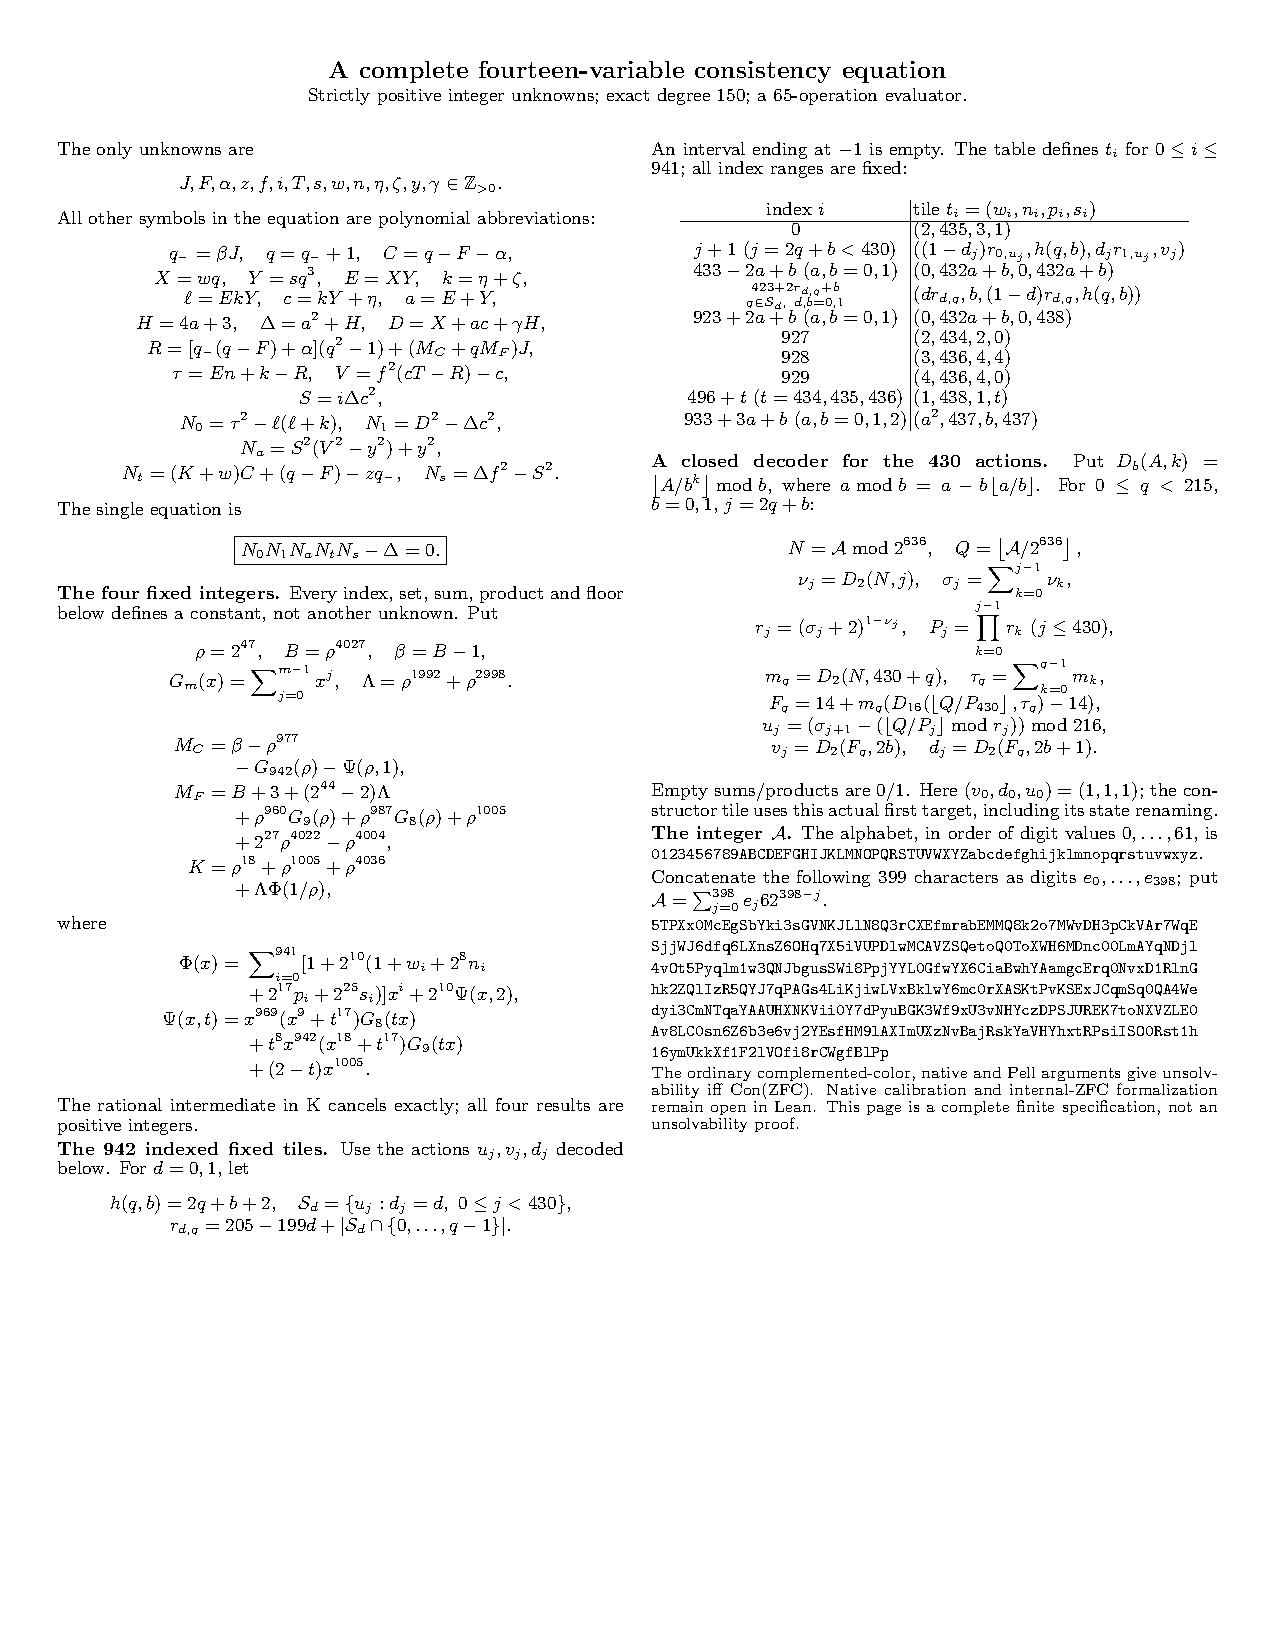
\includepdf[pages=1,pagecommand={\thispagestyle{empty}}]{equation.pdf}
\end{document}
